\documentclass[a4paper, 11pt]{article}
\usepackage[english]{babel}
\usepackage[ansinew]{inputenc}
\usepackage{graphicx}
\usepackage{listings, lstautogobble}
\pagestyle{headings}

\begin{document}
\bibliographystyle{alphadin}

\title{Detection of Nucleoli Using ImageJ}
\author{Nico Hochberger}
\date{November 2014}
\maketitle

\newpage
\tableofcontents

\newpage
\section{Introduction}

\subsection{Preface}
 
\subsection{Objective}

\subsection{Motivation}
Currently nucleoli are detected using an application called
CellProfiler\footnote{http://www.cellprofiler.org}.
While this application yields reliable results, it also takes pretty long to complete
the analysis. Runtimes up to 45 seconds are common.
Due to the fact that CellProfiler is a very general approach, applicable to a
large variety of tasks related to detecting nuclei and nucleoli, the results of
its analysis have to be checked manually to reduce the amount of
false-positives.
In order to analyze the cells, they need to be taken out of the incubator. Yet,
outside the incubator the cells can only be kept alive for a limited timespan.
Considering this, time is a valuable resource and must not be wasted by using a
too general approach.
Consequently, this leads to a more specialized way of analyzing the cells, which
does not do all the analysis performed by CellProfiler, but on the other hand is
much faster and thus helps to prevent cells dying before the analysis is
finished.

\begin{figure}[h]
    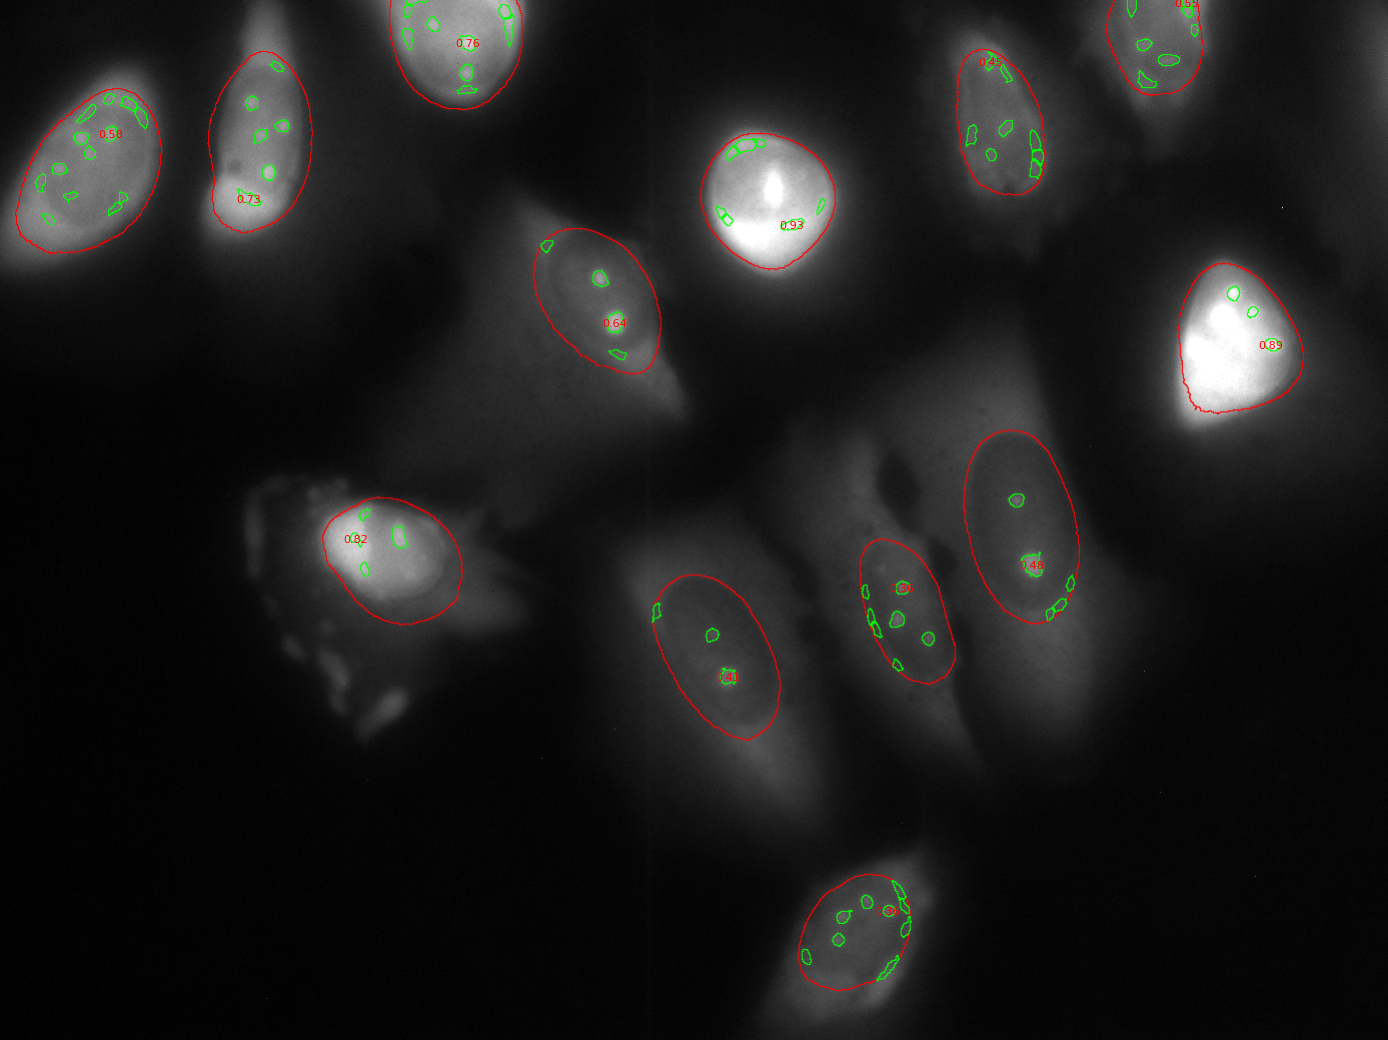
\includegraphics[width=\linewidth]{images/cellprofiler_channel1}
    \caption{Example analysis performed with CellProfiler}
    \label{fig:cellprofiler_example}
\end{figure}

\newpage
\section{Design and Implementation}

\subsection{Requirements}
The application has to meet the following requirements:
\begin{itemize}
  \item \textbf{Reliable nucleoli detection:} Stable and reliable detection of
  nucleoli is the main purpose of the application. Hence, it is supposed to
  detect at least 75\% of the nucleoli CellProfiler can detect. This includes
  a certain degree of stability concerning fuzzy pictures or pictures with
  inequally distributed or diffuse brightnes.
  \item \textbf{Fast analysis:} As the application is tailored to this single
  task, it is expected to detect a suitable amount of nucleoli in only a small
  fraction of the time required by CellProfiler. The topmost time that the
  application may require to complete the analysis of one image is five seconds.
  \item \textbf{Fallback in case of empty nuclei:} Each nucleus is expected to
  containg at least one nucleolus. Yet, this expectation cannot always be
  fulfilled due to potentially damaged nuclei, fuzzy images, or other reasons.
  In this case, the center of the nucleus has to be provided as fallback target.
  \item \textbf{Visualizer:} In order to quickly check the results directly
  after running the analysis and to provide a way to quickly present the results
  to a potential audience, the application has to provide the possibility to be
  configured so that it shows the results as an image. This image has to contain
  all detected neuleoli targets, fallback targets and the regions of interest,
  e.g. the nuclei.
  \item \textbf{Versatility:} Since the appearance of different specimen can
  vary in various ways, all analysis parameters have to be configurable. Among
  others, this includes the minimum and maximum sizes of nuclei and nucleoli.
  The configuration is supposed to be achieved via an understandable,
  interchangeable, text-based file\footnote{Configurable parameters are
  explained in detail in the User's Manual section}.
  \item \textbf{Statistics:} To determine the most suitable parameters for
  different kinds of specimen, another feature may be configured. This
  statistics feature has to include:
  \begin{itemize}
    \item The amount of detected nuclei
    \item The amount of detected nucleoli
    \item Nuclei to nucleoli ratio as percentage
    \item The distance of each detected nucleolus to the center point of the
    containing nuclei and the average distance in pixels
    \item The area of each detected nucleus and the average area in square
    pixels
    \item The area of each detected nucleolus and the average area in square
    pixels
  \end{itemize}
  \item \textbf{Serialization of the results:} All results have to be stored in
  their accordant files in a subfolder \textit{results} of the folder
  containing the original data. In the following, the accordant formats and
  files are described.
  \begin{itemize}
  	\item \textbf{Targets:} Real targets and fallback targets sre to be saved in
  	one txt-file named \textit{targets\_$\langle$timestamp$\rangle$.txt} in the
  	following format:
\begin{lstlisting}[frame=single, caption=Format of results txt-file]
# nucleoli targets
<target number> : [<x-coord>, <y-coord>]
...
# targets in center of empty nuclei
<target number> : [<x-coord>, <y-coord>]
...
\end{lstlisting}

		\textbf{Example:}
\begin{lstlisting}[frame=single, caption=Example of results file]
# nucleoli targets
1 : [468, 43]
2 : [1183, 14]
# targets in center of empty nuclei
3 : [87, 174]
4 : [769, 198]
\end{lstlisting}
  	\item \textbf{Statistics:} The statistics as mentioned above have to be
  	stored in a txt-file named   
  	\textit{statistics\_$\langle$timestamp$\rangle$.txt}. An example of the
  	statistics file can be found in the appendix.
  	\item \textbf{Result image:} The image as it would be displayed by the
  	visualizer has to be stored to a file named
  	\textit{targets\_$\langle$timestamp$\rangle$.$\langle$original
  	image filetype$\rangle$}. See Figure \ref{fig:target_image_example} for an
  	example the image. 
  	\begin{figure}[h]
	    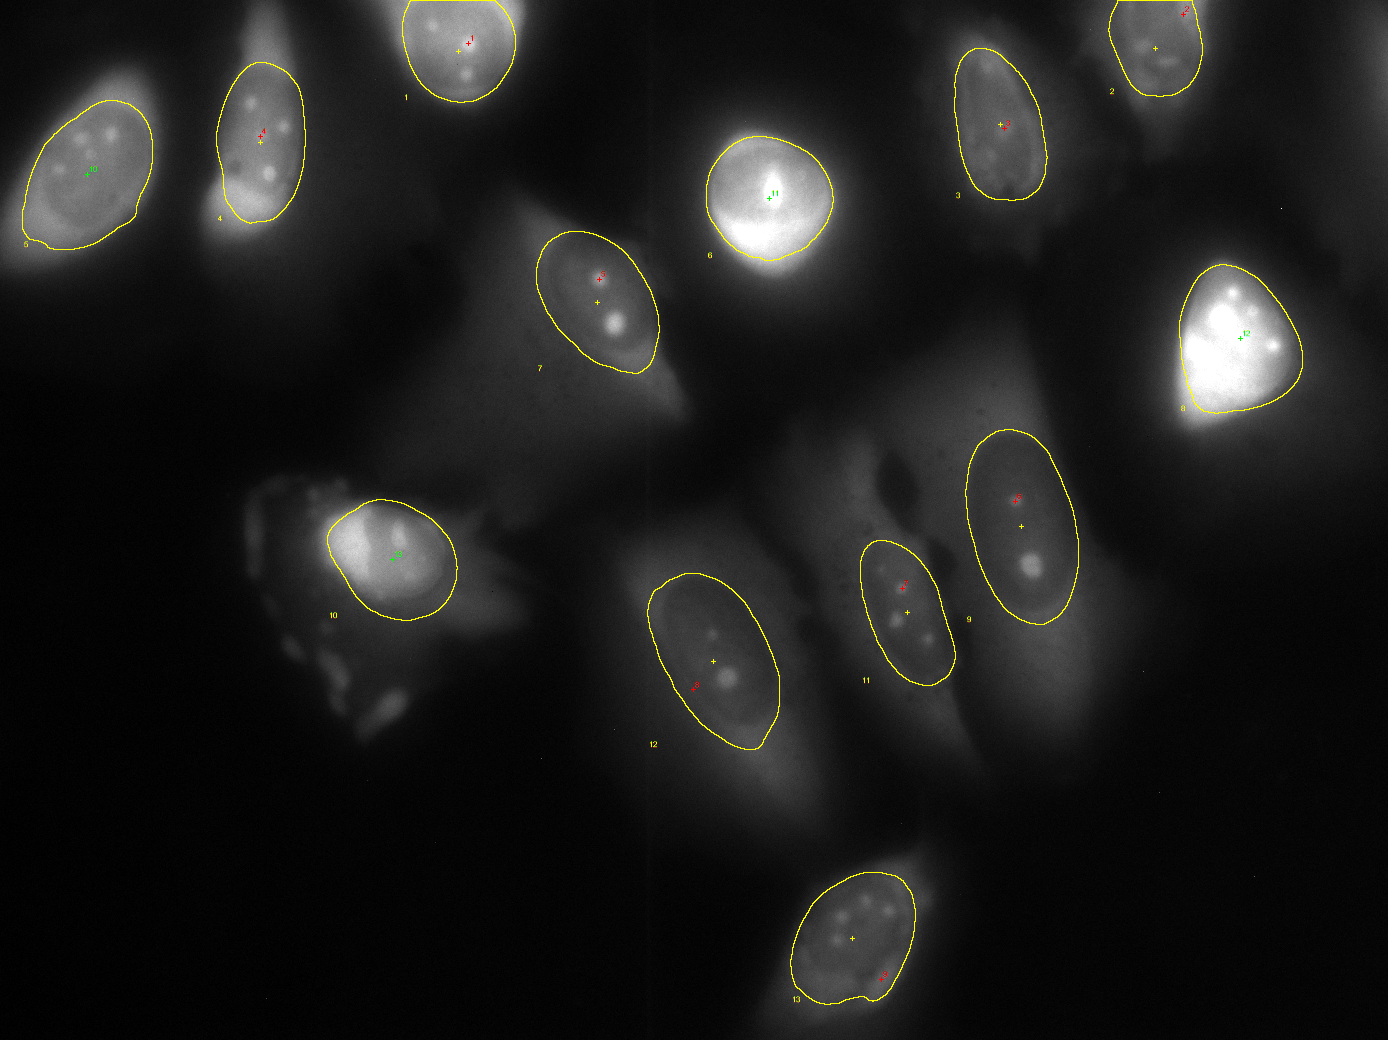
\includegraphics[width=\linewidth]{images/targets_example}
	    \caption{Example of the image containing the results}
	    \label{fig:target_image_example}
	\end{figure}
  \end{itemize}
  \item \textbf{Quick and easy deployment:} The application is supposed to be
  deployed and run as easily as possible. Since the environment and the machines
  this will happen on may vary drastically, a versatile and independent way to
  do this is required. The Java framework delivers this possibility. Hence, the
  application will be developed using Java.
\end{itemize}
\newpage

\section{User's Manual}

\subsection{System Requirements}
As the application is built upon the Java framework, the minimum system
requirements are based on that of the Java framework version 1.7.0\_71
\footnote{Details on the system requirements can be found at:
https://docs.oracle.com/javase/7/docs/webnotes/install/windows/windows-system-requirements.html}.

As it is good practice and vital to the security of any system, the Java
framework should be updated on a regular basis. Thus the requirements will
change with any update.
\subsection{Starting the Application}

\subsection{Configuration}
\subsubsection{General Parameters}
\subsubsection{Improved Image Detection Parameters}
\subsubsection{Structure of Files and Folders}

\newpage
\section{Conclusion and Prospect}
 
\subsection{Conclusion}

\subsection{Prospect}


\newpage
\addcontentsline{toc}{section}{Bibliography}
\bibliography{sources}

\end{document}